% Provenance (never printed): old premiere S material on the structure of the
% Earth from seismology (P and S waves, travel times, the Moho, the shadow zone
% and the core, a reference model); see sources/book2/PROVENANCE.md. Profiles
% from figdata/grade-11/prem_profiles.py, rays and travel times from
% seismic_rays.py, the refraction lines and the problem's readings from
% moho_refraction.py. Lehmann's story and portrait are told in Book 1 (g6
% inside-the-earth): recalled here, not repeated.
\chapter{地震波揭示地球内部}\label{ch:g11:seismic-structure}

1909 年 10 月 8 日，一次地震震动了库帕河谷，
位于克罗地亚萨格勒布东南约 \qty{40}{km} 处。
几个月前，安德里亚·莫霍洛维奇在萨格勒布气象
台安装了一台新地震仪，记录下了整个事件。他随后向其他
台站索取记录，共收集到 41 个台站的记录。
在较远台站的记录中，他发现了一个意外现象：出现了两组
彼此分开的 \omterm{def:g11:seismic-structure:body-waves}{P 波}，一弱一强，按理本应
只有一组。他由这一对波推断，地壳之下的岩石
性质不同，并测定了该界面的深度。本章说明
地震波到达的时刻如何揭示地球的各个分层：
地壳的底部、地核及其液态外核，以及
整个地球内部，由浅入深逐层揭示。
% ledger: herak:kupa-1909, srl:mohorovicic, geotech:moho-1909, kayal:pn-sn

\begin{recall}
地震始于地球内部的一点，即震源；
其正上方的地表点称为震中。地震仪记录地面的
震动，震级度量地震的大小（第 1 册，
七年级）。地球分为地壳、地幔和地核，地核包括液态的
外核和固态的内核。地震波主要有两类：
速度较快的 \omterm{def:g11:seismic-structure:body-waves}{P 波}和速度较慢的 \omterm{def:g11:seismic-structure:body-waves}{S 波}，\omterm{def:g11:seismic-structure:body-waves}{S 波}不能穿过液体
（第 1 册，六年级）。波穿过两种介质之间的界面时，
若其在两种介质中的速度分别为 $v_1$ 和 $v_2$，则发生折射：
$\sin i_1/v_1 = \sin i_2/v_2$，其中角度自界面的
垂线量起（斯涅耳定律；见物理各册）。
\end{recall}

\section{地震波与走时}

\subsection{两类体波}

地震向各个方向发出波动。一部分沿地表传播；
另一部分即体波，穿过地球内部传播，正是
它们揭示了地球内部的情况。

\begin{definition}[P 波；S 波]\label{def:g11:seismic-structure:body-waves}
\emph{P 波}\index{P 波}是一种地震波，它使岩石交替受压与受拉，
岩石沿波的传播方向来回运动。
它可穿过固体、液体和气体，并且是速度最快的地震波，
因此最先到达。\emph{S 波}\index{S 波}使岩石发生剪切，
即岩石沿与波的传播方向成直角的方向运动。它只能穿过固体，
并且比 P 波晚到达。
\end{definition}
% ledger: kayal:p-s

液体能够流动，对形状的改变不产生抵抗，因此无法
传递剪切，这正是 \omterm{def:g11:seismic-structure:body-waves}{S 波}在液体表面被阻断的原因。在大多数
岩石中，\omterm{def:g11:seismic-structure:body-waves}{P 波}的速度约为 \omterm{def:g11:seismic-structure:body-waves}{S 波}的 $\sqrt 3 \approx 1.7$ 倍。
在上地壳中，\omterm{def:g11:seismic-structure:body-waves}{P 波}速度约为 \qty{5.8}{km/s}，\omterm{def:g11:seismic-structure:body-waves}{S 波}
约为 \qty{3.2}{km/s}；紧邻地壳之下，两者分别达到
约 \qty{8.1}{km/s} 和 \qty{4.5}{km/s}。
% ledger: kayal:p-s, kayal:outer-core-liquid, data:prem (vp_surface 5.8, vs_surface 3.2,
% vp_upper_mantle 8.11, vs_upper_mantle 4.49 in figdata/grade-11/prem_profiles.py)

\begin{omfigure}

\includegraphics[width=0.5\linewidth]{images/book2/g11-usgs-seismometer.jpg}

{\small 波多黎各地震台网与 USGS 的地震学家，
于 2020 年 1 月 10 日，在波多黎各西南部安装一台临时地震仪。
照片：Thomas Pratt, USGS（公有领域）。}
\end{omfigure}
% ledger: photo:g11-seismometer

\subsection{走时曲线}

地震到远处台站的距离，用角度来度量：
即地心处震中与台站之间的夹角 $\Delta$，
称为\emph{震中距}\index{震中距}。震中距的一度
沿地表约合 $\qty{111.2}{km}$。
% ledger: earth:Rmean

\begin{definition}[走时；走时曲线]\label{def:g11:seismic-structure:travel-time}
地震波在某台站的\emph{走时}\index{走时}，
即从震源传到该台站所需的时间。
某种波的\emph{走时曲线}\index{走时曲线}，
即其走时对台站震中距的图像。
\end{definition}

台站记录下每种波的到达时刻；若已知地震的发生时刻，
两者之差即为\omterm{def:g11:seismic-structure:travel-time}{走时}。成千上万次地震被成千上万个台站记录，
使\omterm{def:g11:seismic-structure:travel-time}{走时曲线}得到了极为精确的确定。
图中的曲线由
\cref{sec:g11:seismic-structure:model}中的地球参考模型计算得出，而图中的点为
真实地震中观测到的\omterm{def:g11:seismic-structure:travel-time}{走时}。两者在各处相差不超过百分之二，
多数情况下相差不超过一到两秒。

\begin{omfigure}
\begin{tikzpicture}
\begin{axis}[omrecord, width=0.84\linewidth, height=6.4cm, xmin=0, xmax=180, ymin=0, ymax=30,
  xtick={0,20,...,180}, ytick={0,5,...,30},
  xlabel={震中距 $\Delta$（度）}, ylabel={走时（分钟）},
  tick label style={font=\small}, label style={font=\small}, clip=false]
% computed in figdata/grade-11/seismic_rays.py; ledger: data:prem, auspass:surftim
\addplot[omDef, line width=0.9pt] table[x=delta_deg, y=t_min] {figdata/out/grade-11-seismic_rays-ttp.dat};
\addplot[omProp, line width=0.9pt] table[x=delta_deg, y=t_min] {figdata/out/grade-11-seismic_rays-tts.dat};
\addplot[omDef, line width=0.9pt, densely dashed] table[x=delta_deg, y=t_min] {figdata/out/grade-11-seismic_rays-ttpkp.dat};
\addplot[omDef!55, line width=0.9pt, densely dotted] table[x=delta_deg, y=t_min] {figdata/out/grade-11-seismic_rays-ttpkikp.dat};
\addplot[only marks, mark=*, mark size=1.5pt, black] table[x=delta_deg, y=p_min] {figdata/out/grade-11-seismic_rays-observed.dat};
\addplot[only marks, mark=*, mark size=1.5pt, black, unbounded coords=discard] table[x=delta_deg, y=s_min] {figdata/out/grade-11-seismic_rays-observed.dat};
\node[font=\small, text=omProp, anchor=south east] at (axis cs:68,21.2) {S};
\node[font=\small, text=omDef, anchor=north west] at (axis cs:72,11.2) {P};
\node[font=\small, text=omDef, anchor=south, align=center] at (axis cs:158,23.2) {P 波 \\穿过地核};
\fill[black!10] (axis cs:98.5,0) rectangle (axis cs:143.8,3.2);
\node[font=\scriptsize, align=center] at (axis cs:121.1,1.6) {无直达 P 波};
\end{axis}
\end{tikzpicture}

{\small 地表地震产生的 \omterm{def:g11:seismic-structure:body-waves}{P 波}（蓝色）与 \omterm{def:g11:seismic-structure:body-waves}{S 波}（橙色）\omterm{def:g11:seismic-structure:travel-time}{走时曲线}，
依据\omterm{def:g11:seismic-structure:reference-model}{参考地球模型}计算；虚线
与点线为穿过地核的 \omterm{def:g11:seismic-structure:body-waves}{P 波}（点线：内核）。
黑点：观测\omterm{def:g11:seismic-structure:travel-time}{走时}。约 \ang{99} 至
\ang{144} 之间没有 \omterm{def:g11:seismic-structure:body-waves}{P 波}直接到达（阴\omterm{def:g11:seismic-structure:shadow-zone}{影区}）。}
\end{omfigure}

S 曲线比 P 曲线上升得更陡，因此两次到达的时间差
随距离增大。据此
可由单个记录求得地震的距离。

\begin{method}[由 S--P 时差求地震距离]\label{met:g11:seismic-structure:distance}
\begin{enumerate}
  \item 在记录上读出第一个 \omterm{def:g11:seismic-structure:body-waves}{P 波}和第一个 \omterm{def:g11:seismic-structure:body-waves}{S 波}的到达时刻；
        二者之差即为 S--P 时差。
  \item 在\omterm{def:g11:seismic-structure:travel-time}{走时曲线}（或其数据表）上，
        找出 S 曲线比 P 曲线高出该时差时
        所对应的震中距。
  \item 必要时用 $\qty{111.2}{km}$ 每度换算为千米。
\end{enumerate}
若有三个台站，则震中是到三个台站距离
都正确的那一点。
\end{method}

\begin{example}[距离 \ang{60} 的地震]\label{ex:g11:seismic-structure:sp}
在 \ang{60} 处，\omterm{def:g11:seismic-structure:body-waves}{P 波}的\omterm{def:g11:seismic-structure:travel-time}{走时}为 \qty{608}{s}，\omterm{def:g11:seismic-structure:body-waves}{S 波}为 \qty{1101}{s}；
在 \ang{50} 处则为 \qty{536}{s} 和 \qty{967}{s}。某台站记录到
\omterm{def:g11:seismic-structure:body-waves}{S 波}比 \omterm{def:g11:seismic-structure:body-waves}{P 波}晚 \qty{493}{s}（8~分 13~秒）到达，因此该台站距震中
\ang{60}，约为 $60 \times 111.2 \approx
\qty{6670}{km}$。在 \ang{50} 处时差只有 \qty{431}{s}。
\end{example}
% ledger: auspass:surftim

\begin{omfigure}
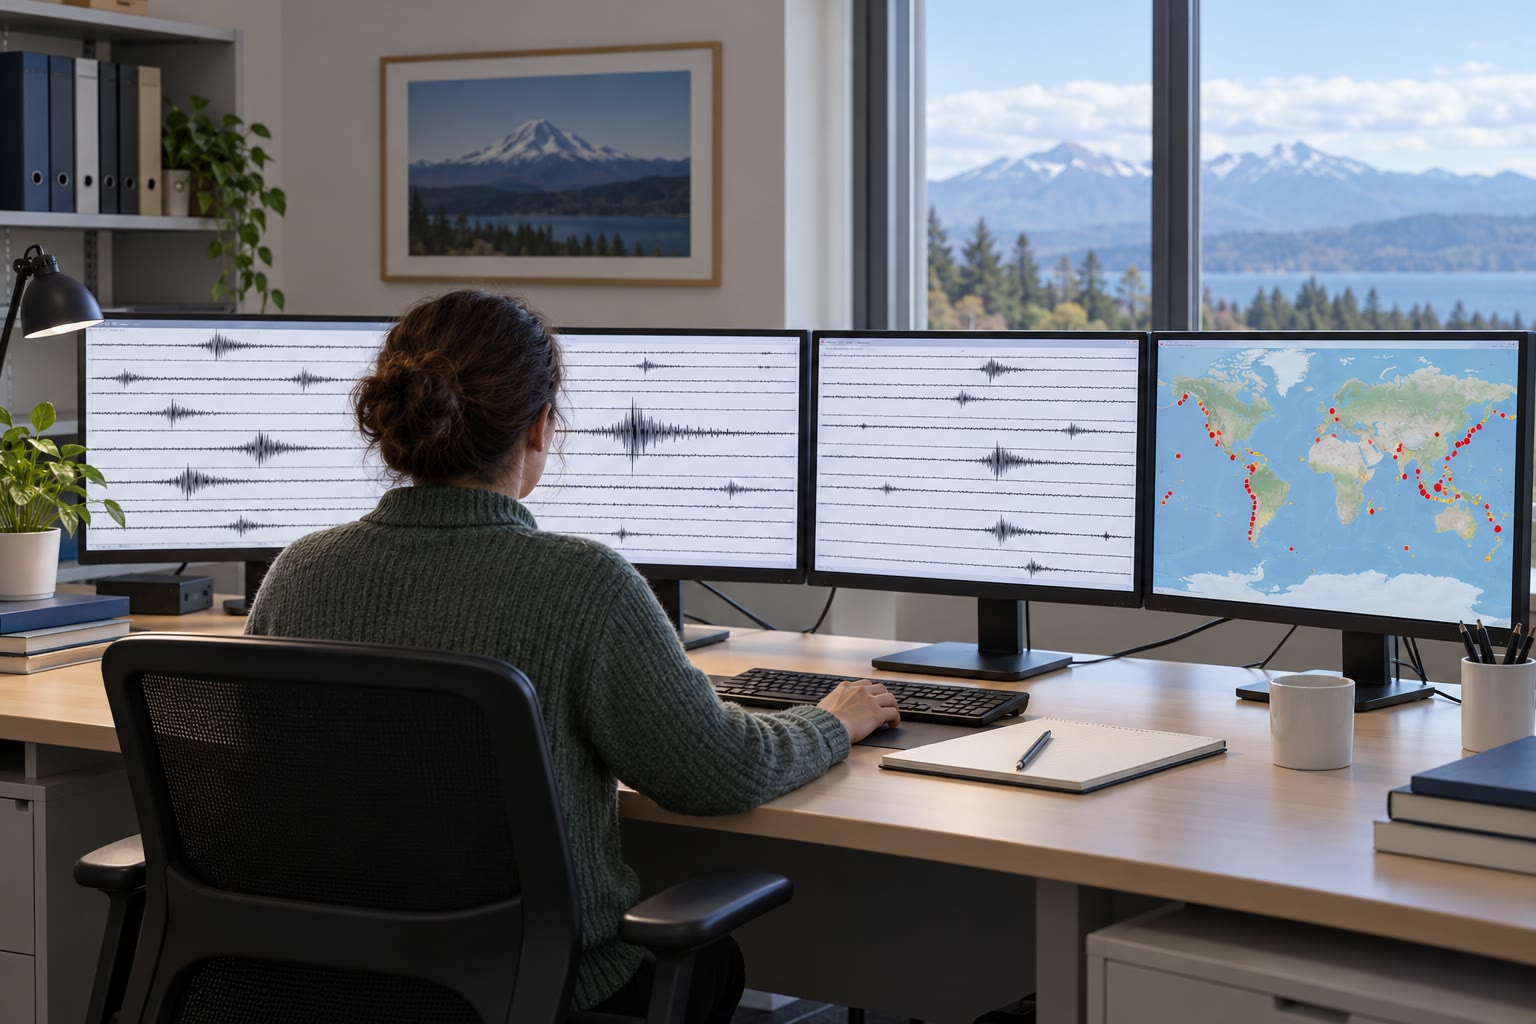
\includegraphics[width=0.66\linewidth]{images/book2/ai/g11-seismology-observatory.jpg}

{\small 在地震台观测站中，多个台站的记录并排显示，
所定位的地震标在世界地图上
（AI 插图）。}
\end{omfigure}

\section{折射与莫霍面}\label{sec:g11:seismic-structure:moho}

\subsection{沿界面传播的波}

在地球内部，地震波的速度随深度变化，多数情况下
是渐变的，但在某些地方是突变的。

\begin{definition}[地震波速不连续面]\label{def:g11:seismic-structure:discontinuity}
地球内部的某一面称为\emph{地震波速不连续面}\index{地震波速不连续面}，
在该面上地震波的速度发生突然变化，
变化发生的厚度远小于波的波长。
\end{definition}

在不连续面处，波的一部分被反射，一部分被折射。设
一层厚度为 $h$ 的介质，其中 \omterm{def:g11:seismic-structure:body-waves}{P 波}的速度为 $v_1$，其下方是一层
速度更大的介质，$v_2 > v_1$。以与竖直方向成 $i$ 角向下传播的射线
在界面处以角度 $r$ 折射，且 $\sin r = (v_2/v_1)\sin
i$，即折射光线偏离竖直方向。当 $\sin i$ 达到 $v_1/v_2$ 时，
折射光线恰好沿界面传播。角
\[
  i_c, \qquad \sin i_c = \frac{v_1}{v_2},
\]
称为\emph{临界角}\index{临界角}。以\omterm{ex:g11:seismic-structure:sp}{临界角}折射的波
沿速度较大一层的顶部以速度 $v_2$ 传播，
并在传播过程中向上层发出波，这些波均以
$i_c$ 角到达地表，形成\emph{首波}\index{首波}。

\begin{omfigure}
\begin{tikzpicture}[x=0.05cm, y=0.05cm, font=\footnotesize, >={Stealth[length=4pt]}]
% geometry from figdata/grade-11/moho_refraction.py: v1 6.2, v2 8.1, h 30 km, ic 49.9 deg
  \fill[omLithGranite!45] (-10,0) rectangle (215,-30);
  \fill[omLithPeridotite!45] (-10,-30) rectangle (215,-48);
  \draw[line width=0.6pt] (-10,0) -- (215,0);
  \draw[line width=0.9pt] (-10,-30) -- (215,-30);
  \node[anchor=west, align=left] at (218,-15) {地壳 \\$v_1 = \qty{6.2}{km/s}$};
  \node[anchor=west, align=left] at (218,-39) {地幔 \\$v_2 = \qty{8.1}{km/s}$};
  \node[anchor=east] at (215,-26) {莫霍面};
  % source and station
  \fill[omDef] (0,0) circle (1.6);
  \node[anchor=south] at (0,1.5) {震源};
  \draw[fill=white] (197,0) -- (203,0) -- (200,5) -- cycle;
  \node[anchor=south] at (200,5) {台站};
  % direct wave
  \draw[->, omProp, line width=0.8pt] (2,-2) -- (196,-2);
  \node[anchor=south, text=omProp] at (100,0.3) {直达波，速度 $v_1$};
  % head wave
  \draw[omDef, line width=0.9pt] (0,0) -- (35.7,-30);
  \draw[->, omDef, line width=0.9pt] (35.7,-30) -- (100,-30);
  \draw[omDef, line width=0.9pt] (100,-30) -- (164.3,-30) -- (200,0);
  \node[anchor=north, text=omDef] at (100,-31) {沿莫霍面以 $v_2$ 传播};
  \foreach \x in {50,70,90,110,130,150} {
    \draw[->, omDef!60, densely dashed] (\x,-30) -- ++(25.5,21.5);
  }
  % critical angle
  \draw[black!60, densely dotted] (35.7,-30) -- (35.7,-8);
  \draw[black!70] (35.7,-18) arc[start angle=90, end angle=130.05, radius=12];
  \node[anchor=south east] at (33,-16) {$i_c$};
  % thickness and critical distance
  \draw[<->] (-6,0) -- (-6,-30);
  \node[anchor=east] at (-7,-15) {$h$};
\end{tikzpicture}

{\small 直达波与\omterm{ex:g11:seismic-structure:sp}{首波}（按比例绘制，地壳厚 \qty{30}{km}
）。\omterm{ex:g11:seismic-structure:sp}{首波}以\omterm{ex:g11:seismic-structure:sp}{临界角} $i_c$ 向下传播，沿地幔顶部运行，
并以 $i_c$ 角返回；沿其在\omterm{def:g11:seismic-structure:moho}{莫霍面}上的整段路径，
它向地表发出波（虚线）。距离小于
$2h\tan i_c$ 的台站都收不到它（此处约 \qty{71}{km}）。}
\end{omfigure}

\begin{proposition}[首波的走时]\label{prop:g11:seismic-structure:head-wave}
若震源位于地表，则距离 $x \ge 2h\tan i_c$ 的台站
在下列时刻收到\omterm{ex:g11:seismic-structure:sp}{首波}：
\[
  t(x) = \frac{x}{v_2} + \frac{2h\cos i_c}{v_1}.
\]
其\omterm{def:g11:seismic-structure:travel-time}{走时曲线}是斜率为 $1/v_2$ 的直线，将其向回延长，
与时间轴相交于\emph{截距时间}\index{截距时间}
$t_i = 2h\cos i_c/v_1$。
\end{proposition}

\begin{proof}
射线沿长为 $h/\cos i_c$ 的斜线下行，
水平推进 $h\tan i_c$；上行时亦然。其间，
它沿界面传播 $x - 2h\tan i_c$。\omterm{def:g11:seismic-structure:travel-time}{走时}为
\[
  t = \frac{2h}{v_1\cos i_c} + \frac{x - 2h\tan i_c}{v_2}
    = \frac{x}{v_2} + \frac{2h}{v_1\cos i_c} - \frac{2h\sin i_c}{v_2\cos i_c}.
\]
由 $1/v_2 = \sin i_c/v_1$，末两项合并为
$\frac{2h}{v_1\cos i_c}\,(1 - \sin^2 i_c) = \frac{2h\cos i_c}{v_1}$.
\end{proof}

直达波在 $x/v_1$ 时刻到达，其曲线是过原点的直线，
比\omterm{ex:g11:seismic-structure:sp}{首波}直线更陡。靠近震源时，直达波先到；
远处则因\omterm{ex:g11:seismic-structure:sp}{首波}大部分路程以较大的速度传播，
\omterm{ex:g11:seismic-structure:sp}{首波}将超过直达波。

\begin{proposition}[交叉距离]\label{prop:g11:seismic-structure:crossover}
\omterm{ex:g11:seismic-structure:sp}{首波}在超过\emph{交叉
距离}\index{交叉距离}之后先于直达波到达：
\[
  x_c = 2h\sqrt{\frac{v_2 + v_1}{v_2 - v_1}}.
\]
\end{proposition}

\begin{proof}
两者同时到达的条件是 $x/v_1 = x/v_2 + 2h\cos i_c/v_1$，即
$x\,(v_2 - v_1)/(v_1 v_2) = 2h\cos i_c/v_1$，于是 $x = 2h\cos i_c\,v_2/(v_2 -
v_1)$。注意到 $\cos i_c = \sqrt{1 - v_1^2/v_2^2} = \sqrt{(v_2 - v_1)(v_2 +
v_1)}/v_2$，因此 $x = 2h\sqrt{(v_2 + v_1)(v_2 - v_1)}/(v_2 - v_1) =
2h\sqrt{(v_2 + v_1)/(v_2 - v_1)}$。超过该距离后，\omterm{ex:g11:seismic-structure:sp}{首波}的直线
斜率较小，先到达。
\end{proof}

\begin{omfigure}
\begin{tikzpicture}
\begin{axis}[omrecord, width=0.78\linewidth, height=5.6cm, xmin=0, xmax=300, ymin=0, ymax=50,
  xtick={0,50,...,300}, xlabel={距震中的距离 (\unit{km})}, ylabel={走时 (\unit{s})},
  tick label style={font=\small}, label style={font=\small}, clip=false]
% computed in figdata/grade-11/moho_refraction.py (critical_km 71.4, crossover_km 164.6, intercept_s 6.23)
\addplot[omProp, line width=0.9pt] table[x=x, y=tdirect] {figdata/out/grade-11-moho_refraction-model.dat};
\addplot[omDef, line width=0.9pt, restrict x to domain=71:300] table[x=x, y=thead] {figdata/out/grade-11-moho_refraction-model.dat};
\addplot[omDef, densely dashed, restrict x to domain=0:72] table[x=x, y=thead] {figdata/out/grade-11-moho_refraction-model.dat};
\draw[black!50, densely dotted] (axis cs:164.6,0) -- (axis cs:164.6,26.5);
\node[font=\scriptsize, anchor=north] at (axis cs:164.6,0) {$x_c$};
\fill (axis cs:0,6.23) circle (1.5pt);
\draw[black!60] (axis cs:0.8,6.6) -- (axis cs:6,12);
\node[font=\scriptsize, anchor=south west, inner sep=1pt] at (axis cs:5,12) {$t_i = \qty{6.2}{s}$};
\node[font=\small, text=omProp, anchor=south east] at (axis cs:250,41) {直达波};
\node[font=\small, text=omDef, anchor=north west] at (axis cs:235,33) {首波};
\end{axis}
\end{tikzpicture}

{\small 上一图中地壳的直达波与\omterm{ex:g11:seismic-structure:sp}{首波}\omterm{def:g11:seismic-structure:travel-time}{走时}。
\omterm{ex:g11:seismic-structure:sp}{首波}直线向回延长（虚线）后，与时间轴相交于
\omterm{prop:g11:seismic-structure:head-wave}{截距时间}；超过\omterm{prop:g11:seismic-structure:crossover}{交叉距离} $x_c \approx
\qty{165}{km}$ 后，\omterm{ex:g11:seismic-structure:sp}{首波}先到达。}
\end{omfigure}

\subsection{地壳的底部}

\begin{definition}[莫霍面]\label{def:g11:seismic-structure:moho}
\emph{莫霍洛维奇不连续面}\index{莫霍洛维奇不连续面}，或
\emph{莫霍面}\index{莫霍面}，是位于地壳底部的
\omterm{def:g11:seismic-structure:discontinuity}{地震波速不连续面}，在此处 \omterm{def:g11:seismic-structure:body-waves}{P 波}速度从至多约 \qty{7}{km/s}
跃升至约 \qty{8}{km/s}，即最上地幔中的速度。
\end{definition}
% ledger: kayal:pn-sn, data:prem (6.8 -> 8.11 at 24.4 km)

\begin{history}[莫霍洛维奇与两种 P 波，1909 年]
安德里亚·莫霍洛维奇（1857--1936）在 1909 年
地震的记录中发现，超过某一距离——一般在 100 至
\qty{150}{km}——一种较弱但较快的 \omterm{def:g11:seismic-structure:body-waves}{P 波}先于强 \omterm{def:g11:seismic-structure:body-waves}{P 波}到达。
他将其解释为：该波曾穿过地壳之下速度较快的岩石，
他将两种波分别命名为 Pg（地壳中的直达波）和 Pn（
沿地幔顶部传播的\omterm{ex:g11:seismic-structure:sp}{首波}），对 \omterm{def:g11:seismic-structure:body-waves}{S 波}亦如此，
并由此推算出两层的速度及二者界面的深度。
Pn 波的传播速度约为 \qty{8.0}{km/s}，即最上
地幔的速度。他于 1910 年发表的论文证明了地壳与地幔
有所不同，该界面以他的名字命名。
\end{history}
% ledger: kayal:pn-sn, srl:mohorovicic

\begin{method}[由走时图确定莫霍面的深度]\label{met:g11:seismic-structure:moho}
\begin{enumerate}
  \item 以首达时间为纵轴、震中
        距离为横轴作图。
  \item 画出直达波的直线（过原点）及\omterm{ex:g11:seismic-structure:sp}{首波}的直线，
        二者斜率分别为 $1/v_1$ 与 $1/v_2$。
  \item 将\omterm{ex:g11:seismic-structure:sp}{首波}直线向回延长至时间轴，它与时间轴相交于
        \omterm{prop:g11:seismic-structure:head-wave}{截距时间} $t_i$。
  \item 由 $\sin i_c = v_1/v_2$，地壳厚度为
        $h = \dfrac{v_1\,t_i}{2\cos i_c}$.
\end{enumerate}
\end{method}

\begin{example}[厚 \qty{30}{km} 的地壳]\label{ex:g11:seismic-structure:moho}
已知 $v_1 = \qty{6.2}{km/s}$，$v_2 = \qty{8.1}{km/s}$，$\sin i_c = 0.765$，
$i_c \approx \ang{49.9}$，$\cos i_c \approx 0.644$。\omterm{prop:g11:seismic-structure:head-wave}{截距时间}为
\qty{6.23}{s}，由此得 $h = 6.2 \times 6.23/(2 \times 0.644) \approx
\qty{30}{km}$。\omterm{ex:g11:seismic-structure:sp}{首波}首次到达地表的距离为
$2h\tan i_c \approx \qty{71}{km}$，
超过 $x_c = 60\sqrt{14.3/1.9} \approx \qty{165}{km}$ 后，\omterm{ex:g11:seismic-structure:sp}{首波}先于直达波到达。
\end{example}
% values computed in figdata/grade-11/moho_refraction.py (ic_deg 49.9, critical_km 71.4, crossover_km 164.6)

用此方法在全球测得，\omterm{def:g11:seismic-structure:moho}{莫霍面}在大洋底之下仅约
\qty{5}{km}。在大陆之下，\omterm{def:g11:seismic-structure:moho}{莫霍面}
平均深约 \qty{41}{km}：在地壳被拉伸的地区约 \qty{30}{km}，
在山脉之下超过 \qty{45}{km}，在最高山脉之下深达约
\qty{100}{km}。地壳是一层薄薄的外壳：即使是
\qty{41}{km}，也不到地球半径的百分之一。
% ledger: usgs:crust-thickness, cm95:crust, kayal:discontinuities

\section{地核}

\subsection{弯曲的射线}

在地幔中，地震波的速度随深度增加。向下传播的射线穿过越来越快的岩石，
根据斯涅耳定律，每前进一段，射线就比前一段更偏离竖直方向，
路径因而弯曲，并折返向地表。射线向下拐得越深，
从震源出发后返回地表的位置就离震源越远。
图中所示射线是用
\omterm{def:g11:seismic-structure:reference-model}{参考地球模型}的速度计算的。

\begin{omfigure}
\begin{tikzpicture}
\begin{axis}[width=0.66\linewidth, height=0.66\linewidth, axis equal image, hide axis,
  xmin=-1.18, xmax=1.18, ymin=-1.18, ymax=1.2, clip=false]
% computed in figdata/grade-11/seismic_rays.py; ledger: data:prem
\fill[omLithPeridotite!25] (axis cs:0,0) circle [radius=1];
\fill[omSea!45] (axis cs:0,0) circle [radius=0.5462];
\fill[omSea!80] (axis cs:0,0) circle [radius=0.1917];
\addplot[black, line width=0.6pt, domain=0:360, samples=181] ({cos(x)}, {sin(x)});
\addplot[black!60, line width=0.4pt, domain=0:360, samples=181] ({0.5462*cos(x)}, {0.5462*sin(x)});
\addplot[black!60, line width=0.4pt, domain=0:360, samples=91] ({0.1917*cos(x)}, {0.1917*sin(x)});
\addplot[omDef, line width=0.6pt] table {figdata/out/grade-11-seismic_rays-praysmantle.dat};
\addplot[omDef!70!black, line width=0.6pt] table {figdata/out/grade-11-seismic_rays-prayscore.dat};
\addplot[omProp, line width=0.6pt] table {figdata/out/grade-11-seismic_rays-srays.dat};
% P shadow zone: 98.5 to 143.8 degrees from the source (right); S beyond 102.7 (left)
\addplot[black!80, line width=3pt, domain=-53.8:-8.5, samples=40] ({1.04*cos(x)}, {1.04*sin(x)});
\addplot[omProp!60, line width=3pt, domain=192.7:270, samples=40] ({1.04*cos(x)}, {1.04*sin(x)});
\fill[omDef] (axis cs:0,1) circle (2pt);
\node[font=\footnotesize, anchor=south] at (axis cs:0,1.04) {震源};
\node[font=\footnotesize, anchor=west, align=left] at (axis cs:1.07,-0.42) {无直达 P 波 \\(\ang{99}--\ang{144})};
\node[font=\footnotesize, anchor=east, align=right] at (axis cs:-1.07,-0.62) {无直达 S 波 \\\ang{103} 以远};
\node[font=\footnotesize, text=omDef, anchor=south west] at (axis cs:0.55,0.8) {P};
\node[font=\footnotesize, text=omProp, anchor=south east] at (axis cs:-0.55,0.8) {S};
\node[font=\scriptsize] at (axis cs:-0.5,-0.62) {地幔};
\node[font=\scriptsize] at (axis cs:-0.3,0.2) {外核};
\draw[black!70] (axis cs:-0.1,-0.06) -- (axis cs:-0.26,-0.22);
\node[font=\scriptsize, anchor=north east, inner sep=1pt] at (axis cs:-0.24,-0.22) {内核};
\end{axis}
\end{tikzpicture}

{\small 震源位于地球顶部时的射线，用参考模型速度计算。右侧：
在地幔中折返的 \omterm{def:g11:seismic-structure:body-waves}{P 波}射线，最远至约 \ang{99}；穿过地核、
在约 \ang{144} 以远射出的 \omterm{def:g11:seismic-structure:body-waves}{P 波}射线。两者之间，没有 \omterm{def:g11:seismic-structure:body-waves}{P 波}射线直接到达。
左侧：\omterm{def:g11:seismic-structure:body-waves}{S 波}射线在地幔中折返，没有任何一条穿过液态外核，
直达 \omterm{def:g11:seismic-structure:body-waves}{S 波}在约 \ang{103} 以远
不再到达。}
\end{omfigure}

\subsection{影区与液态外核}

1906 年，地震学家奥尔德姆注意到，在地球另一侧记录到的 \omterm{def:g11:seismic-structure:body-waves}{P 波}
比预期时刻晚到，并提出地球中心存在一个中心核，\omterm{def:g11:seismic-structure:body-waves}{P 波}在其中传播得较慢。
1912 年，古登堡发现，\omterm{def:g11:seismic-structure:body-waves}{P 波}不能到达约 \ang{105} 至 \ang{143} 之间的
一整段距离，并在刚超过 \ang{143} 处出现强烈的到达；
1914 年，他确定地核顶部位于
\qty{2900}{km} 深处。
% ledger: kayal:discontinuities, kayal:shadow

\begin{definition}[影区]\label{def:g11:seismic-structure:shadow-zone}
地震波的\emph{影区}\index{影区}是指该波无法从
震源直接到达的震中距范围，原因是地核使其
弯曲或阻挡。
\end{definition}

射线可以解释这一现象。恰好在地核之上折返的 \omterm{def:g11:seismic-structure:body-waves}{P 波}射线，
在距震源约 \ang{100} 处回到地表。射线稍陡一些便进入地核，
在那里 \omterm{def:g11:seismic-structure:body-waves}{P 波}速度从 \qty{13.7}{km/s} 骤降至约 \qty{8.1}{km/s}：
根据斯涅耳定律，射线向竖直方向\emph{偏折}，穿过地核后在远得多的地方射出，
即约 \ang{144} 以远。在地幔中折返的 \omterm{def:g11:seismic-structure:body-waves}{P 波}射线，
与穿过地核的 \omterm{def:g11:seismic-structure:body-waves}{P 波}射线，都不会落在两者之间。
在参考模型中，\omterm{def:g11:seismic-structure:body-waves}{P 波}\omterm{def:g11:seismic-structure:shadow-zone}{影区}从 \ang{98.5} 延伸到
\ang{143.8}，与古登堡所测的 \ang{105}--\ang{143} 相近。
% ledger: kayal:shadow, data:prem (vp_above_cmb 13.72, vp_below_cmb 8.06); computed in
% figdata/grade-11/seismic_rays.py (shadow_start_deg 98.5, shadow_end_pkp_deg 143.8)

\omterm{def:g11:seismic-structure:body-waves}{S 波}提供的信息更多。没有任何 \omterm{def:g11:seismic-structure:body-waves}{S 波}穿过外核：外核不能传递剪切波，
因此它是液态的。于是，在参考模型中，直达 \omterm{def:g11:seismic-structure:body-waves}{S 波}
在约 \ang{103} 以远不再到达，
即整个地球另一侧都收不到直达 \omterm{def:g11:seismic-structure:body-waves}{S 波}。
% ledger: kayal:outer-core-liquid; computed in figdata/grade-11/seismic_rays.py (s_direct_max_deg 102.7)

\begin{definition}[核幔边界；内核边界]\label{def:g11:seismic-structure:core}
\emph{核幔边界}\index{核幔边界}是固态地幔与液态外核之间的\omterm{def:g11:seismic-structure:discontinuity}{地震波速不连续面}，
位于 \qty{2891}{km} 深处；在该处 \omterm{def:g11:seismic-structure:body-waves}{P 波}速度由约
\qty{13.7}{km/s} 降至约 \qty{8.1}{km/s}，\omterm{def:g11:seismic-structure:body-waves}{S 波}在此停止传播。
\emph{内核边界}\index{内核边界}位于 \qty{5150}{km} 深处，
将液态外核与固态内核分开；在该处 \omterm{def:g11:seismic-structure:body-waves}{P 波}速度由约
\qty{10.4}{km/s} 跃升至约
\qty{11.0}{km/s}。
\end{definition}
% ledger: data:prem, prem:cmb, prem:icb (Book 3 rows); values in figdata/grade-11/prem_profiles.py

\omterm{def:g11:seismic-structure:shadow-zone}{影区}并非完全寂静：其中仍有微弱的 \omterm{def:g11:seismic-structure:body-waves}{P 波}到达。1936 年，英格·莱曼
用固态内核解释了这些波，因为在内核中 \omterm{def:g11:seismic-structure:body-waves}{P 波}传播得更快（见第 1 册，六年级）。
射线图清楚地显示了这一点。\omterm{def:g11:seismic-structure:body-waves}{P 波}射线到达内核后，
在速度向上跃升处像在\omterm{def:g11:seismic-structure:moho}{莫霍面}那样偏离竖直方向，
并比其他射线更早地从地核射出：在参考模型中，
穿过内核的射线从约 \ang{121} 起到达地表，
位于\omterm{def:g11:seismic-structure:shadow-zone}{影区}之内（\omterm{def:g11:seismic-structure:travel-time}{走时}图中的虚线曲线）。
% ledger: nbi:lehmann-1936 (Book 1 row), kayal:lehmann; computed in
% figdata/grade-11/seismic_rays.py (pkikp_min_deg 121.4)

\section{参考地球模型}\label{sec:g11:seismic-structure:model}

综合数百万个\omterm{def:g11:seismic-structure:travel-time}{走时}，即可得到 \omterm{def:g11:seismic-structure:body-waves}{P 波}和 \omterm{def:g11:seismic-structure:body-waves}{S 波}在各深度的速度。
波速取决于岩石及其密度，而地球的总质量决定其平均
密度；二者结合，
便可得到各深度的密度。
% ledger: data:prem, prem:constraints (Book 3 row)

\begin{definition}[参考地球模型]\label{def:g11:seismic-structure:reference-model}
称\emph{参考地球模型}\index{参考地球模型}为一张表，给出
随深度变化的 \omterm{def:g11:seismic-structure:body-waves}{P 波}速度、\omterm{def:g11:seismic-structure:body-waves}{S 波}速度和密度，
在各方向上相同，并经选取使其与观测到的地震波\omterm{def:g11:seismic-structure:travel-time}{走时}
及地球质量相符。
\end{definition}

应用最广的是初步\omterm{def:g11:seismic-structure:reference-model}{参考地球模型}（PREM），由
A.~M.~德齐温斯基和 D.~L.~安德森于 1981 年发表。本章的射线与\omterm{def:g11:seismic-structure:travel-time}{走时}
均由该模型算出，例如 \ang{60} 处的 \omterm{def:g11:seismic-structure:body-waves}{P 波}\omterm{def:g11:seismic-structure:travel-time}{走时}为
\qty{607}{s}，观测值为 \qty{608}{s}。
% ledger: data:prem, auspass:surftim; computed in figdata/grade-11/seismic_rays.py (p_60_s 607.2)

\begin{omfigure}
\begin{tikzpicture}
\begin{axis}[omrecord, width=0.86\linewidth, height=6.2cm, xmin=0, xmax=6371, ymin=0, ymax=14.5,
  xtick={0,1000,...,6000}, ytick={0,2,...,14}, scaled x ticks=false,
  xticklabel style={/pgf/number format/1000 sep={\,}},
  xlabel={深度（\unit{km}）}, ylabel={速度（\unit{km/s}）或密度（\unit{g/cm^3}）},
  tick label style={font=\small}, label style={font=\small}, clip=false]
% computed in figdata/grade-11/prem_profiles.py; ledger: data:prem
\addplot[omDef, line width=0.9pt] table[x=depth, y=vp] {figdata/out/grade-11-prem_profiles-profile.dat};
\addplot[omProp, line width=0.9pt] table[x=depth, y=vs] {figdata/out/grade-11-prem_profiles-profile.dat};
\addplot[black, line width=0.9pt, densely dashed] table[x=depth, y=rho] {figdata/out/grade-11-prem_profiles-profile.dat};
\foreach \d in {670,2891,5149.5} {\edef\temp{\noexpand\draw[black!40, densely dotted] (axis cs:\d,0) -- (axis cs:\d,14.5);}\temp}
\node[font=\scriptsize, anchor=south, align=center] at (axis cs:2891,14.5) {核幔 \\边界};
\node[font=\scriptsize, anchor=south, align=center] at (axis cs:5149.5,14.5) {内核 \\边界};
\node[font=\scriptsize, anchor=south] at (axis cs:670,14.5) {\qty{670}{km}};
\node[font=\small, text=omDef, anchor=south] at (axis cs:1800,12.4) {P 波速度};
\node[font=\small, text=omProp, anchor=south] at (axis cs:1800,7.0) {S 波速度};
\node[font=\small, anchor=north] at (axis cs:1800,4.5) {密度};
\node[font=\scriptsize, align=center] at (axis cs:4000,1.9) {无 S 波：\\液态};
\end{axis}
\end{tikzpicture}

{\small 初步\omterm{def:g11:seismic-structure:reference-model}{参考地球模型}中 \omterm{def:g11:seismic-structure:body-waves}{P 波}和 \omterm{def:g11:seismic-structure:body-waves}{S 波}的速度及密度随深度的变化
（德齐温斯基和安德森，1981 年）。虚线标出\omterm{def:g11:seismic-structure:moho}{莫霍面}以下的主要不连续面，
\omterm{def:g11:seismic-structure:moho}{莫霍面}埋深太浅，
在此比例尺下无法显示。}
\end{omfigure}

从顶部开始读取该模型：
\begin{itemize}
  \item 地壳的 \omterm{def:g11:seismic-structure:body-waves}{P 波}速度为 5.8 至 \qty{6.8}{km/s}，
        止于\omterm{def:g11:seismic-structure:moho}{莫霍面}（本平均模型中为 \qty{24.4}{km}）；
  \item 地幔中，波速随深度增大，并伴有较小的突变，
        其中最大的突变位于 \qty{400}{km} 和 \qty{670}{km} 附近；
  \item 在 \qty{2891}{km} 处，\omterm{def:g11:seismic-structure:body-waves}{S 波}速度降为零，\omterm{def:g11:seismic-structure:body-waves}{P 波}速度
        下降超过 \qty{5}{km/s}：液态外核；
  \item 在 \qty{5150}{km} 处，\omterm{def:g11:seismic-structure:body-waves}{S 波}重新出现：固态内核，
        半径为 \qty{1220}{km}。
\end{itemize}
% ledger: data:prem (discontinuities in figdata/grade-11/prem_profiles.py)

密度由地壳中的 \qty{2.6}{g/cm^3} 升至
地幔底部的 \qty{5.6}{g/cm^3}，随后在地核顶部跃升至
\qty{9.9}{g/cm^3}，并在地心达到 \qty{13.1}{g/cm^3}。
整个模型的平均密度为 \qty{5.5}{g/cm^3}，是地壳岩石密度的两倍：
地球深部，尤其是地核，由密度远大于地表的
物质构成。地核约占地球质量的
三分之一。
% ledger: data:prem, prem:cmb, prem:centre (Book 3 rows); computed in
% figdata/grade-11/prem_profiles.py (mean_density 5.52; core mass fraction 0.32)

\section{练习}

\begin{exercise}[$\star$]\label{exo:g11:seismic-structure:1}
写出 \omterm{def:g11:seismic-structure:body-waves}{P 波}与 \omterm{def:g11:seismic-structure:body-waves}{S 波}之间的两点区别。哪一种波先被
地震仪记录到？为什么？
\end{exercise}

\begin{exercise}[$\star$]\label{exo:g11:seismic-structure:2}
某台站位于距震中 \ang{40} 处。沿地表量取，
其距离为多少？另一台站距震中 \qty{8900}{km}，
其角距离是多少度？
\end{exercise}

\begin{exercise}[$\star$]\label{exo:g11:seismic-structure:3}
在 \ang{40} 处观测到的\omterm{def:g11:seismic-structure:travel-time}{走时}，\omterm{def:g11:seismic-structure:body-waves}{P 波}为 \qty{456}{s}，
\omterm{def:g11:seismic-structure:body-waves}{S 波}为 \qty{822}{s}。将其换算为分钟和秒，并求出 S--P
延迟。
\end{exercise}

\begin{exercise}[$\star$]\label{exo:g11:seismic-structure:4}
\omterm{def:g11:seismic-structure:body-waves}{P 波}速度为 \qty{6.0}{km/s} 的地壳覆盖在
\omterm{def:g11:seismic-structure:body-waves}{P 波}速度为 \qty{8.0}{km/s} 的地幔之上。计算\omterm{ex:g11:seismic-structure:sp}{临界角}。
\end{exercise}

\begin{exercise}[$\star$]\label{exo:g11:seismic-structure:5}
在参考模型中，\omterm{def:g11:seismic-structure:core}{核幔边界}位于深 \qty{2891}{km} 处，
\omterm{def:g11:seismic-structure:core}{内核边界}位于深 \qty{5150}{km} 处；地球半径为
\qty{6371}{km}。求外核的厚度、地核的半径，以及
地核半径与地球半径之比。
\end{exercise}

\begin{exercise}[$\star\star$]\label{exo:g11:seismic-structure:6}
观测到的 S--P 延迟：\ang{20} 处为 \qty{224}{s}，\ang{30} 处为 \qty{298}{s}，
\ang{40} 处为 \qty{366}{s}，\ang{50} 处为 \qty{431}{s}，以及
\ang{60} 处为 \qty{493}{s}。某台站记录到 \omterm{def:g11:seismic-structure:body-waves}{S 波}比 \omterm{def:g11:seismic-structure:body-waves}{P 波}晚 6~分钟 6~秒，
该地震距台站多少度？合多少千米？
为什么单个台站无法确定地震的位置？
\end{exercise}

\begin{exercise}[$\star\star$]\label{exo:g11:seismic-structure:7}
利用\cref{exo:g11:seismic-structure:4}中的速度，以及厚
\qty{35}{km} 的地壳，计算距震中 \qty{200}{km} 处台站的直达波与
\omterm{ex:g11:seismic-structure:sp}{首波}的\omterm{def:g11:seismic-structure:travel-time}{走时}。哪一个先到达？
\end{exercise}

\begin{exercise}[$\star\star$]\label{exo:g11:seismic-structure:8}
对\cref{exo:g11:seismic-structure:7}中的地壳，计算临界距离
$2h\tan i_c$ 和\omterm{prop:g11:seismic-structure:crossover}{交叉距离}。检验
\cref{exo:g11:seismic-structure:7}的答案是否一致。
\end{exercise}

\begin{exercise}[$\star\star$]\label{exo:g11:seismic-structure:9}
洋底下方有一层厚 \qty{6}{km} 的地壳，其中 \omterm{def:g11:seismic-structure:body-waves}{P 波}速度为
\qty{6.5}{km/s}，其下为速度 \qty{8.0}{km/s} 的地幔。计算\omterm{ex:g11:seismic-structure:sp}{临界
角}、\omterm{prop:g11:seismic-structure:head-wave}{截距时间}和\omterm{prop:g11:seismic-structure:crossover}{交叉距离}。为什么在洋底下找到\omterm{def:g11:seismic-structure:moho}{莫霍面}，
台站之间必须比在大陆下
靠得更近？
\end{exercise}

\begin{exercise}[$\star\star$]\label{exo:g11:seismic-structure:10}
最底层地幔中的 P 射线速度为 \qty{13.7}{km/s}，
它以与法线成 \ang{30} 的入射角到达\omterm{def:g11:seismic-structure:core}{核幔边界}。边界以下
\omterm{def:g11:seismic-structure:body-waves}{P 波}速度为 \qty{8.06}{km/s}。计算折射光线的角度，并判断
折射光线是向法线偏折还是远离法线？用此解释为什么
进入地核的 P 射线会在远离震中处射出。
\end{exercise}

\begin{exercise}[$\star\star$]\label{exo:g11:seismic-structure:11}
在地球参考模型中，\omterm{def:g11:seismic-structure:body-waves}{P 波}沿过地心的直线向下传播，
到达地球另一侧的对应点需 \qty{1210}{s}。若
沿整条直径（\qty{12742}{km}）以 \qty{13.7}{km/s} 的速度（即地幔底部的 \omterm{def:g11:seismic-structure:body-waves}{P 波}速度）传播，
需要多长时间？奥尔德姆由这类延迟得出了什么结论？
\end{exercise}

\begin{exercise}[$\star\star\star$]\label{exo:g11:seismic-structure:12}
(1) 由\cref{prop:g11:seismic-structure:head-wave}，证明
地壳的厚度为
\[
  h = \frac{t_i\,v_1 v_2}{2\sqrt{v_2^2 - v_1^2}}.
\]
(2) 将其应用于 $t_i = \qty{6.23}{s}$、$v_1 = \qty{6.2}{km/s}$ 和
$v_2 = \qty{8.1}{km/s}$。
\end{exercise}

\begin{exercise}[$\star\star\star$]\label{exo:g11:seismic-structure:13}
地球的平均密度为 \qty{5.52}{g/cm^3}。将地球视为
由半径为 \qty{3480}{km}、密度均匀为 $\rho_c$ 的地核，
外部包有密度均匀、为 \qty{4.45}{g/cm^3} 的地幔与地壳（取
地球参考模型的平均值）。(1) 地核体积占地球体积的几分之几？(2) 求
$\rho_c$。(3) 将其与地球参考模型中地核顶部的
密度 \qty{9.9}{g/cm^3} 以及地壳的密度相比较。
\end{exercise}

\begin{exercise}[$\star\star\star$]\label{exo:g11:seismic-structure:14}
古登堡的 \omterm{def:g11:seismic-structure:body-waves}{P 波}\omterm{def:g11:seismic-structure:shadow-zone}{影区}从 \ang{105} 延伸至 \ang{143}。(1) 给出其
沿地表的界限（以千米计）。(2) 在球面上，到某点的角距离介于
$a$ 与 $b$ 之间的区域，占整个球面的比例为 $(\cos a - \cos
b)/2$。问给定一次地震时，地表中收不到
直接 \omterm{def:g11:seismic-structure:body-waves}{P 波}的部分占多大比例？(3) 为什么每次地震都有各自的
\omterm{def:g11:seismic-structure:shadow-zone}{影区}？
\end{exercise}

\begin{exercise}[$\star\star\star$]\label{exo:g11:seismic-structure:15}
在某高山山脉下方，折射测量得到 $v_1 =
\qty{6.3}{km/s}$、$v_2 = \qty{8.1}{km/s}$，以及\omterm{prop:g11:seismic-structure:head-wave}{截距时间}为
\qty{9.5}{s}。(1) 计算该处地壳的厚度。(2) 若地壳厚 \qty{30}{km}，
且波速相同，其\omterm{prop:g11:seismic-structure:head-wave}{截距时间}应为多少？
(3) 与陆壳的平均厚度相比较。
\end{exercise}

\section{问题：寻找莫霍面}

\begin{problem}[{周末问题——由十五个台站确定地壳的深度}]
\label{pb:g11:seismic-structure:1}
% readings computed in figdata/grade-11/moho_refraction.py (part stations; invented region,
% v1 6.2, v2 8.1, h 30 km, reading errors of up to 0.1 s); ledger: kayal:pn-sn, usgs:crust-thickness
一次小地震发生在大陆之下极浅的深度处。
十五个台站沿一条从震中出发的直线布设，记录
第一个 \omterm{def:g11:seismic-structure:body-waves}{P 波}的到达时间，以及在能够读出时的第二个
波的到达时间。下表读数为虚构，但按实际测量会得到的结果计算，
精确到十分之一秒。Pg 是穿过地壳传播的波，
Pn 则是沿地幔顶部传播的波。

\begin{center}
\small
\begin{tabular}{|c|c|c||c|c|c|}
\hline
距离（\unit{km}） & Pg（\unit{s}） & Pn（\unit{s}） & 距离（\unit{km}） & Pg（\unit{s}） & Pn（\unit{s}） \\ \hline
20 & 3.3 & --- & 180 & 29.0 & 28.5 \\ \hline
40 & 6.5 & --- & 200 & 32.3 & 30.9 \\ \hline
60 & 9.7 & --- & 220 & --- & 33.3 \\ \hline
80 & 12.8 & 16.2 & 240 & --- & 35.8 \\ \hline
100 & 16.1 & 18.6 & 260 & --- & 38.3 \\ \hline
120 & 19.3 & 21.1 & 280 & --- & 40.8 \\ \hline
140 & 22.6 & 23.6 & 300 & --- & 43.2 \\ \hline
160 & 25.8 & 26.0 & & & \\ \hline
\end{tabular}
\end{center}

\medskip
\noindent\textbf{第一部分——直达波。}
\begin{enumerate}
  \item 在方格纸上作出 Pg 与 Pn 的\omterm{def:g11:seismic-structure:travel-time}{走时}随距离变化的图（\qty{1}{cm}
        分别代表 \qty{20}{km} 与 \qty{5}{s}）。Pg 各点呈何种排列？
  \item 为什么 Pg 直线几乎经过原点？
  \item 利用 20 与 \qty{200}{km} 处的台站，计算 Pg 直线的斜率，
        单位为秒每千米。
  \item 由此推出地壳中 \omterm{def:g11:seismic-structure:body-waves}{P 波}的速度 $v_1$。
  \item 若地壳继续延伸，Pg 波在
        \qty{300}{km} 处的台站上将于何时到达？
\end{enumerate}

\medskip
\noindent\textbf{第二部分——折射波。}
\begin{enumerate}[resume]
  \item 利用 100 与 \qty{300}{km} 处的台站，计算 Pn 直线的斜率
        以及地壳之下 \omterm{def:g11:seismic-structure:body-waves}{P 波}的速度 $v_2$。
  \item 将 $v_2$ 与莫霍洛维奇测得的 Pn 波速度
        约 \qty{8.0}{km/s} 进行比较。地壳之下是何种岩石？
  \item 计算\omterm{ex:g11:seismic-structure:sp}{临界角} $i_c$。
  \item 距离小于 \qty{80}{km} 的台站均未记录到 Pn 波。利用
        \cref{prop:g11:seismic-structure:head-wave}，解释为何存在一个
        可以记录到\omterm{ex:g11:seismic-structure:sp}{首波}的最小距离。
  \item 在 80 与 \qty{160}{km} 之间，Pn 波晚于 Pg 波到达。为何仍能
        被记录到？
\end{enumerate}

\medskip
\noindent\textbf{第三部分——交叉点。}
\begin{enumerate}[resume]
  \item 由表可知，首个到达的波由 Pg 变为 Pn 时，
        位于哪两个台站之间？
  \item 分别写出两条直线的方程，
        取 \qty{20}{km}（Pg）与 \qty{100}{km}（Pn）处的数据点。
  \item 计算两直线相交处的距离。
  \item 超过 \qty{200}{km} 后，没有台站能将 Pg 作为独立的波记录。
        \qty{250}{km} 处的台站首先记录到何种波，于何时记录到？
\end{enumerate}

\medskip
\noindent\textbf{第四部分——\omterm{def:g11:seismic-structure:moho}{莫霍面}的深度。}
\begin{enumerate}[resume]
  \item 将 Pn 直线反向延长至时间轴，其\omterm{prop:g11:seismic-structure:head-wave}{截距时间}
        $t_i$ 为多少？
  \item 计算 $\cos i_c$，并利用
        \cref{met:g11:seismic-structure:moho} 求出地壳厚度 $h$。
  \item 验算：取此 $h$，利用
        \cref{prop:g11:seismic-structure:crossover} 计算\omterm{prop:g11:seismic-structure:crossover}{交叉距离}，并与
        第 13 题的结果比较。
  \item 再次验算：计算临界距离 $2h\tan i_c$，并与
        记录到 Pn 波的最近台站比较。
  \item 地震学家给出的 $h$ 仅精确到几千米。为何
        无法给出更精确的数值？
  \item 作出结论：此地区的\omterm{def:g11:seismic-structure:moho}{莫霍面}位于何种深度？就大陆而言，
        此处地壳属薄还是厚？
\end{enumerate}
\end{problem}
